\section{Study 1: Policies}
% general motivation - why do we investigate this?
We start out with the exploration of psychological factors for the design of password policies. We were motivated by the fact that at this point, policies are a one-fits-all solution that evidently does not work in the same ways for all users: Shay \etal observed that subjective usability ratings for policies differed among participants \cite{Shay2012CorrectHorseBatteryStaple, Shay2014CanLongPasswordsBeSecureAndUsable}. For instance, about 40\% of their participants found it difficult to create a password under a ``3class16'' policy, but another 40\% found it easy \cite{Shay2014CanLongPasswordsBeSecureAndUsable}. Following the general discourse and related results from privacy research, we hypothesized that an individual's personality might be responsible for their attitudes towards one policy or another. Therefore, our goal in this project was to explore such associations between personality traits and policy preference. 
%GOALS: explore associations between big-five traits and password selection under different policies, both on usability and security metrics. Investigate the effects of using a non-traditional password policy based on emojis. user preference for one policy or another. explorative study so no p-values.
\subsection{Method}
% general methodology
Our study was completely exploratory, because the literature did not allow us to derive narrow hypotheses. Since personality traits are nuanced, we opted for an online survey to collect a larger sample. Personality was assessed in the Five-Factor Model. We opted for the BFI-K construct by Rammstedt and John \cite{Rammstedt2005BFI}, because it is freely available in German. Moreover, with its 21 items, the time to fill out the questionnaire is kept reasonably low. 
Participants were asked to create several passwords in a row, i.e. the study followed a within-groups protocol. Here, we evaluated three different password policies: a traditional (3class12), an uncommon (2word12), and a novel policy (emoji12) that required the selection of at least one emoji through a graphical user interface (more on emojis in chapter \ref{chap:emojipasswords}). The reason for this choice was that the policies are different enough to serve as levels of the independent variable ``policy''. Participants assessed the ``difficulty to create'' a password for each policy. Moreover, we had them rank the policies by their personal preference, so the choice of 3class12, 2word12, and emoji12 would help them spot and judge the differences easily. 

\subsubsection{Structure and Tasks}
The study was divided into 3 overall parts. In the first part, participants were briefed about privacy details of the study and they provided demographic background information. Then they proceeded to the personality questionnaire before they were asked to perform three experimental tasks. Each consisted of creating a password and assessing the difficulty with agreement levels on the three items \textit{``It was difficult to create a password that meets the requirements''}, \textit{``I found the password requirements bothersome''}, and \textit{``It was easy to create a \textit{new} password''}. Agreement was measured on a five-point scale ranging from ``Strongly disagree'' to ``Strongly agree''. Inversely keying the items as well double encoding makes the data more robust against implausible responses. 

The order of the policies was counterbalanced to mitigate order effects, we recorded the order as a control variable. We chose an online-banking scenario for all three selections. The first prompt was to create a password to protect an online banking account. Secondly, participants were told that someone had gained access to their account and the bank locked them out. As a security precaution, they had to reset their first password. The last task description explained that their password had expired after one year and they need to reset it again. This storyline was designed to fulfill the \textit{realistic threat} principle proposed by Krol \etal (see Section \ref{sec:rw:principles-experiments}) \cite{Krol2016ExperimentDesign}. 

We used SosciSurvey, a standard survey tool, to collect the responses. The dynamic parts involving password selection were embedded in iframes. To match the data from the survey tool and the iframe we used URL query parameters containing the response ID. We asked participants to switch to a desktop browser to avoid styling glitches and unexpected behavior from the prototypes. %Auto-complete was prevented in any case

\subsubsection{Recruiting and Demographic Background}
We recruited participants through posts on social networks and by sending out the invitation link in a university-wide newsletter (more than 5000 recipients). To incentivize participation, we announced a raffle of five shopping vouchers with a value of 20€ each. At this point, 222 people had started participation. After drop-out and plausibility checks, the remaining sample size was $N=164$. As expected, the age distribution was narrow: our sample consisted mostly of students in their mid-twenties \average 24.7 (SD=5.5). 79 respondents were female, 83 male, and 2 preferred not to answer. In the background screener, 65 people (40\%) indicated to possess formal training in computer science or information technology. We also requested self-reported assessments on password behaviors. Here we found that 40\% reuse passwords without modification, 32\% reuse them with modifications or with a mnemnoic technique. 17\% often create new passwords. In terms of management strategy, the majority (53\%) tries to memorize passwords. 11\% use a password manager or generator. Written cues served as aid for 10\% of respondents, and 16\% write passwords down on analog media, while 21\% use electronic files. Interestingly, the distribution of coping strategies is very close to survey findings gathered with more diverse samples \cite{CSID2012PasswordHabits}. Hence, we believe to have caught a representative snapshot of password behavior.

\subsubsection{Statistical Analyses}
For statistical analyses, we consulted the StabLab\footurl{http://www.stablab.stat.uni-muenchen.de/}{30.01.2018} to identify suitable methods. After a revision of the collected data and the necessary assumption checks, the associations were explored with additive models (AM). Their advantage over linear regression is more flexible for non-linear associations \footurl{https://en.wikipedia.org/wiki/Additive_model}{30.01.2018}. The \textit{mgcv} package for R was used to calculate the models.

Scores on the Big-Five sub-dimensions served as independent variables, i.e. the predictors in the regression models. \textit{Openness} is coded with five items, while the remaining four dimensions were assessed with four items. The agreement levels for each item were mapped to numeric values from 1 to 5. The score on each sub-dimension is the sum of agreement levels. To better estimate effect sizes, we control for gender, age and IT proficiency in the models. 
\subsubsection{Method Limitations}
The method, albeit carefully executed, faces a few limitations regarding the interpretability. First, the sample was fairly homogeneous, because participants were mostly between 20 and 28 years old and have an academic background. However, personality traits are not age dependent \ar?. Our study was strongly focused on individual preferences and usability perceptions of different policies, so only a within-groups design was feasible. However, in real-life password selection, users rarely select three passwords in a row. The choice of our storyline still makes confident about the ecological validity \cite{Fahl2013EcologicalValidityPasswordStudy}. The repeated measures design did not allow us to measure the policies' influence on password memorability, which we have to postpone to another study. At this stage, the preference was more valuable for our exploration than memorability effects. Besides, we briefed participants to fill out the survey on a desktop PC or a similar device. We cannot guarantee that all participants followed this instruction, which might have had an effect on their password selection \cite{Melicher2016UsabilityMobileTextPasswords}. 

% we had to redeploy the prototype.
Finally, we unfortunately made a mistake in the deployment of the emoji-based policy. Instead of 12 characters, it required participants to select 16 characters beside the emoji. We realized this fact by looking at descriptive statistics during the course of the study, because the policy performed significantly worse than the other two. We re-deployed the emoji-based policy immediately after we had realized the error. Consequently, we had to remove the data for the creation difficulty and ranking in cases 1-61, reducing the overall sample size to 103. Nonetheless, the sample size is sufficiently large to investigate medium to strong effects. 

%- we started out with emoji16, but made the switch to emoji12 (after 43 participants), because emoji16 received the most negative feedback, but it was mostly due to the length. data removed for ranking (1-61) and difficulty to create (1-43). 

\subsection{Results}
Overall, associations between personality and creation difficulty were moderate. In the following, we only describe non-trivial and interesting associations. 


\begin{table}
\begin{center}
\begin{tabular}{l c c c }
\hline
 & emoji12 & 2word12 & 3class12 \\
\hline
(Intercept)               & $9.99^{***}$ & $7.04^{***}$ & $6.26^{*}$ \\
                          & $(2.35)$     & $(0.75)$     & $(2.52)$   \\
Age                       & $0.02$       &              & $-0.05$    \\
                          & $(0.06)$     &              & $(0.06)$   \\
GenderFemale              & $0.91$       & $1.35^{*}$   & $-0.46$    \\
                          & $(0.58)$     & $(0.66)$     & $(0.61)$   \\
ITNo                      & $-0.10$      & $0.60$       & $0.21$     \\
                          & $(0.59)$     & $(0.66)$     & $(0.63)$   \\
Extraversion              & $-0.05$      &              & $-0.01$    \\
                          & $(0.08)$     &              & $(0.08)$   \\
Conscientiousness         & $0.01$       &              & $0.08$     \\
                          & $(0.09)$     &              & $(0.10)$   \\
Neuroticism               & $-0.22^{*}$  &              & $0.05$     \\
                          & $(0.09)$     &              & $(0.09)$   \\
emojiPos2                 & $0.52$       &              &            \\
                          & $(0.65)$     &              &            \\
emojiPos3                 & $0.23$       &              &            \\
                          & $(0.63)$     &              &            \\
%EDF: s(Agreeableness)     & $3.27$       & $2.77$       & $2.02$     \\
%                          & $(4.11)$     & $(3.48)$     & $(2.55)$   \\
%EDF: s(Openness)          & $2.50$       & $1.79$       & $1.53$     \\
%                          & $(3.11)$     & $(2.24)$     & $(1.89)$   \\
twoWordPos2               &              & $-0.38$      &            \\
                          &              & $(0.74)$     &            \\
twoWordPos3               &              & $-0.07$      &            \\
                          &              & $(0.73)$     &            \\
%EDF: s(Age)               &              & $1.81$       &            \\
%                          &              & $(2.25)$     &            \\
%EDF: s(Extraversion)      &              & $1.52$       &            \\
%                          &              & $(1.87)$     &            \\
%EDF: s(Conscientiousness) &              & $3.32$       &            \\
%                          &              & $(4.14)$     &            \\
%EDF: s(Neuroticism)       &              & $1.53$       &            \\
%                          &              & $(1.88)$     &            \\
threeClassPos2            &              &              & $1.19$     \\
                          &              &              & $(0.66)$   \\
threeClassPos3            &              &              & $0.77$     \\
                          &              &              & $(0.69)$   \\
\hline
AIC                       & 591.89       & 615.92       & 604.37     \\
%BIC                       & 635.73       & 668.02       & 642.01     \\
%Log Likelihood            & -280.17      & -289.22      & -288.64    \\
Deviance                  & 772.78       & 899.67       & 890.95     \\
Deviance explained        & 0.15         & 0.21         & 0.10       \\
%Dispersion                & 7.41         & 8.89         & 8.37       \\
R$^2$                     & 0.04         & 0.08         & 0.00       \\
GCV score                 & 8.47         & 10.44        & 9.36       \\
Num. obs.                 & 119          & 119          & 119        \\
Num. smooth terms         & 2            & 6            & 2          \\
\hline
\multicolumn{4}{l}{\scriptsize{$^{***}p<0.001$, $^{**}p<0.01$, $^*p<0.05$}}
\end{tabular}
\caption{GAM summary of creation difficulty}
\label{table:coefficients}
\end{center}
\end{table}

medium associations between extraversion, agreeableness, and neuroticism (basically the other three dimensions that were not useful before), but control variables are associated to a larger degree.

emoji policy similar results as traditional policies, i.e. it is wortwhile to experiment with it

\paragraph{Descriptives and Hypothesis Tests}
creation difficulty: Repeated measures linear mix model ANOVA. random intercept to account for the fact that people generally rate policy usability low. baseline (any could be chosen) emoji 12.

emoji \average 7.89 (in [3;15] range), 2word12 + 0.12, 3class12 - 0.70 (easier)
serial positioning effects do make a difference, but it also appears trivial in the overall sample.
summary: no big difference between policies and ranking. (this is what makes the remainder more exciting, because a closer look at the data brings out how the numbers come to be)


\paragraph{Creation Difficulty}
% gender
Female participants reported more difficulties for emoji12 ($\beta=0.91$) and 2word12 ($\beta=1.35$). 
for 3class12 correlation was smaller ($\beta=-0.46$) and pointed in the opposite direction.
% it background
IT background revealed interesting effects too: emoji12 ($\beta=-0.10$) trivial, 3class12 ($\beta=0.21$) weak, 2word12 ($\beta=0.61$) medium. it looks as though people with higher IT knowledge struggle with a word-based policy, potentially because it is much less common in the wild. 
% order of the policy
If you factor in the order of the policy, the results look clearer. if emoji12 and 3class12 were shown in position 2, creation was more reported to be more difficult emoij12-2 ($\beta=0.52$), 3class12-2 ($\beta=1.19$) 
% age
we observed non-linear associations between age and creation difficulty, but the small age range forbids us to make conclusive inferences from our data.


\begin{figure}
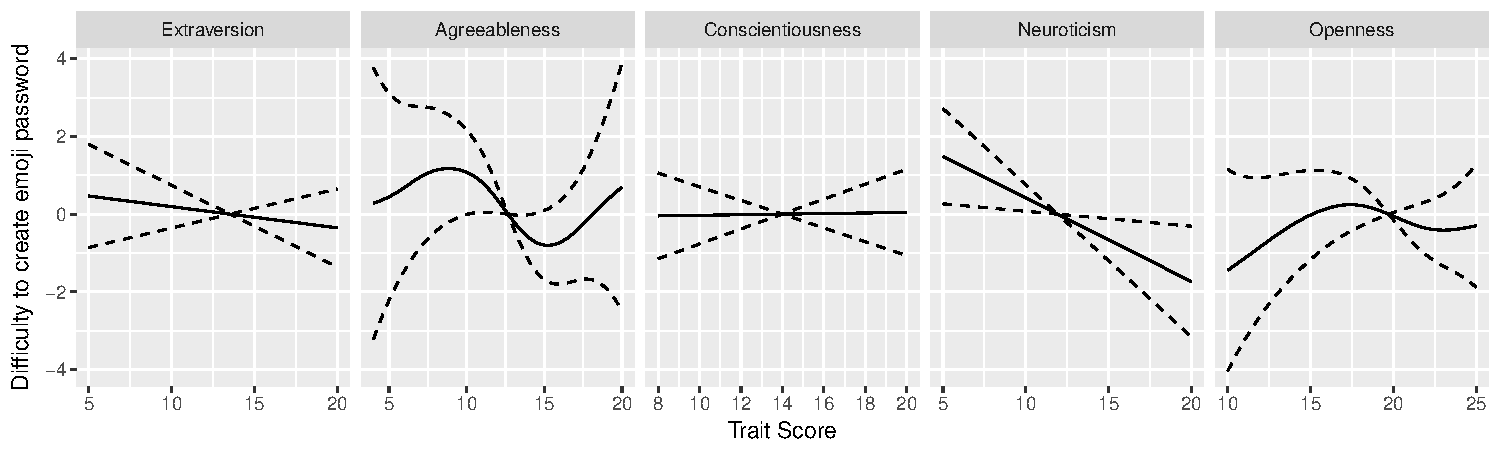
\includegraphics[width=\linewidth]{personality/dc-emoji-b5}
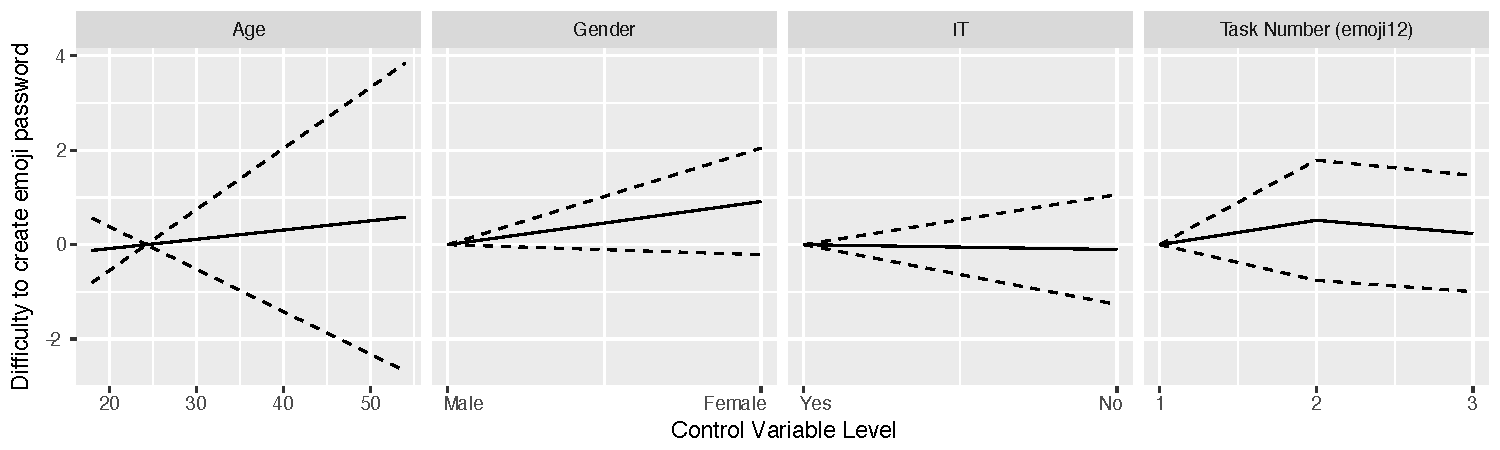
\includegraphics[width=\linewidth]{personality/dc-emoji-control-mod}
\caption{\label{fig:personality:dc-emoji-b5}Associations between predictors and difficulty to create a password under the emoji12 policy. Visualizations of the General Additive Model (gam).}
\end{figure}
%emoji personality
mostly non-linear associations for the emoij12 policy (see Figure \ref{fig:personality:dc-emoji-b5})
neuroticism weak linear association emoji12 ($\beta=-0.22$), i.e. it was slightly easier for people with higher neuroticism scores (this is a great result, albeit weak. neurotic people are by defintion more \textit{emotional}, and emojis seem to cater to this trait.)
agreeableness weak non linear, and interesting curve (up and down) for emoji12
openness weak non linear, but too little data to conclusively decide. 
% 2word12 personality
effects not as clear as for the emoji policy. highly open people report slightly less difficulty to create a 2word12 password.

% 3class12
linear associations are negligible for extraversion, conscientiousness, and neuroticism. 
non-linear associations for agreeableness and openness. at value around 15 (from 20) the difficulty seems to increase (hard to interpret this finding). People with agreeableness scores of 18 and greater find it more difficult to create a 3class12 password by up to 1.5 points. Openness is inversely correlated here. the more open the participant was, the more likely they found it easy to create a 3class12 password. 


\paragraph{Ranking}
logistic additive regression %https://web.stanford.edu/~hastie/Papers/AdditiveLogisticRegression/alr.pdf
did policy X land on top spot ? yes = 1, no = 1. thus, no encompasses the two other options.
Logit model. see timo's work to better understand what's going on. 

\begin{table}
	\centering
	\caption{\label{tab:pws_pers:distribution-binary-ranks} Distribution of binary rankings of the three available policies. Evidently, 3class12 was ranked best in most cases. }
	\begin{tabular}{llll}
		~ 			& emoji12	& 2word12 	& 3class12 \\ \hline\hline
		1st rank	& 18		& 12		& 67 \\
		other rank 	& 80 		& 85 		& 31 \\ \hline
		n			& 98		& 98		& 98		 
	\end{tabular}
\end{table}


% predictors: demography and structure
strong effects. the probability of a non-IT person putting emoji12 at the top is $exp(\beta–{IT-0}=9.87)$, so around ten times higher. only one IT-person ranked emoji12 first. (this fits to the finding that non-IT people found it easier to create an emoji12 password).
% order of policies 
the order in which policies were displayed also produced a notable effect. If emoji12 is shown in 2nd $exp(\beta–{emoji-pos2}=0.27)$ or 3rd position $exp(\beta–{emoij-pos3}=0.76)$, the likelihood to rate it the best policy slightly decreases. Other positionings, as well as age-related preferences, were inconclusive.

% personality
generally weak associations.
extraversion, weak linear effect regarding 2word12. likelihood to put 2word12 first decreases with higher extraversion scores $exp(\beta–{E-1}=0.82)$. for agreeableness both linear and non-linear effects are visible; higher scores increase chances to vote emoji12 first $exp(\beta–{A-1}=1.28)$. openness or conscientiousness have negligible, random associations. for neuroticism we lack data in edge cases (low or high trait scores) to draw conclusions. %there are more results in the BA, but I do not really see the point of reporting all the details of inconclusive results


\paragraph{Password selection}

\todo{create a emoiji selection histogram}. In essence, some emoji were strongly preferred, e.g. the red heart and the ``pouting face''. analyze: what were the usability ratings/rankings of those who picked the heart vs. the pouting face, i.e. are emojis with a positive connotation used by people who are happy that they can select an emoji password? I guess there are significant effects here. 

\subsection{Learnings}
It could have been useful to include a recall test à la ``which passwords do you still remember after filling out the personality questionnaire?'' 

%TODO re-read the discussion section, because the findings are a bit higher level and more understandable
Most interesting finding: Non-IT people significantly less likely to put emoji policy first. s

emoji (negatively) associated with emotional stability, i.e. less stable people who are more emotional in either direction were more positive towards emojis.

non linear associations probably explicable by other variables, e.g. intercorrelation -- 
\todo{discuss the personality traits and associations, try to explain them.}

demographics play a role - (careful now, cowboy): policies could be tailored to gender. but i'm kind of reluctant to put this argument forward. at least IT background could be considered a factor for the policy. a personalized policy would make it more difficult for horizontal attacks because the policy is unpredictable.

mutually exclusive effects for ranking are clear because of the binary nature.

wild idea: if positioning influences the favorability of policies, one could leverage this. like anchoring and decoy (chose your own policy of the three). commitment and consistency as well (commit to your policy, create a strong password to be consistent with your commitment.)